\subsubsection{Trabajo de preparación}

\begin{figure}[ht]
    \centering
    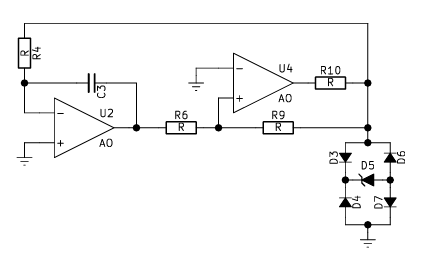
\includegraphics[width=0.5\textwidth]{generador-de-funciones.png}
    \caption{Generador de funciones}
    \label{fig:generador-funciones}
\end{figure}

\paragraph{Para el circuito de la figura \ref{fig:generador-funciones}, diseñar con el fin de obtener una oscilación de frecuencia 5.0kHz.\\}

Llamaremos a la salida del astable $V_{C}$, a la entrada positiva del astable $V_p$ y a la salida del integrador $V_{T}$

Tenemos que la salida $V_{C}$ viene dada por los valores de los diodos y del zener, de modo que 

\begin{equation}
    V_{C} = V_{Z} + 2 V_{D}
\end{equation}

Llamaremos a las entradas del amplificador U4 $V^-$ y $V^+$, el voltaje en $V^+$ viene dado por

\begin{equation*}
    V^+ = \frac{R_6}{R_6 + R_7} V_C + \frac{R_7}{R_6 + R_7} V_T
\end{equation*}

Despejando $V_T$ de la ecuación

\begin{equation*}
    V_T = \frac{R_6 + R_7}{R_7} V^+ - \frac{R_6}{R_7} V_C
\end{equation*}

Pero el voltaje $V^- = 0$ ya que está conectado a la referencia y $V^+ = V^-$ por lo tanto

\begin{equation}
    V_T = - \frac{R_6}{R_7} V_C
\end{equation}

Se utilizarán el diodo zener 1N4734A y los diodos 1N4007, por lo que

\begin{align*}
    V_Z &= 5.80 V \\
    V_D &= 1.00 V
\end{align*}

Por tanto

\begin{equation*}
    V_{C} = \pm 7.80V
\end{equation*}

Para el diseño no se pide ningún valor especifico para la magnitud de la señal triangular en el diseño, por lo tanto se puede escoger cualquier valor para $R_6$ y $R_7$ siempre y cuando $V_T$ no alcance el voltaje de saturación del amplificador. Por simplicidad se utilizará $R_6 = R_7$

por tanto 

\begin{equation*}
    V_T = - V_C
\end{equation*}

\begin{align}
    V_C= 6.9V \rightarrow V_T = -7.8V \\
    V_C = -6.9V \rightarrow V_T = 7.8V
\end{align}

Para cumplir con la condición de frecuencia primero hay que tomar en cuenta el tiempo de retardo de la señal debido al slew rate, el cual viene dado por la expresión

\begin{equation*}
    T_{SR} = \frac{2(V_Z + 2 V_D)}{SR}
\end{equation*}

De la hoja de datos del amplificador $\mu A741$ tenemos que $SR = 0.5 V\mu s$, por tanto

\begin{equation*}
    T_{SR} = \frac{2 \cdot 6.9}{0.5} = 27.6 \mu s
\end{equation*}

Y tenemos que el periodo viene dado por 

\begin{equation*}
    T = T_1 + T_2 + T_{SR}
\end{equation*}

Para este caso $T_1 = T_2$ por tanto la expresión se vuelve

\begin{equation*}
    T = 2 \cdot T_1 + T_{SR}
\end{equation*}

despejando $T_1$

\begin{equation*}
    T_1 = \frac{T - T_{SR}}{2} = \frac{200 - 27.6}{2} \mu S = 86.2 \mu s
\end{equation*}

Entonces de la ecuacion \ref{eq:t1} tenemos

\begin{equation*}
    86.2 \mu s = \frac{2\cdot V_T}{V_C} RC
\end{equation*}

despejando R

\begin{equation}
    R = 86.2 \times10 ^{-6} \frac{V_C}{2 \cdot V_T \cdot C}
\end{equation}

Si $C=10nF$ entonces

\begin{equation}
    R = 4.3k\Omega
\end{equation}

La resistencia $R_{10}$ es para proteger al amplificador debido a que los diodos fijan el voltaje de salida y se debe asegurar que la corriente en la salida sea lo suficientemente pequeña, por lo tanto se escogerá un valor de

\begin{equation}
    R_{10} = 1k\Omega
\end{equation}

\subsubsection{Simulación}

\paragraph{Simular el circuito diseñado y verificar las especificaciones, reportar las formas de ondas de interés para evidenciar el funcionamiento del circuito} 

\begin{ilustracion}[ht]
    \centering
    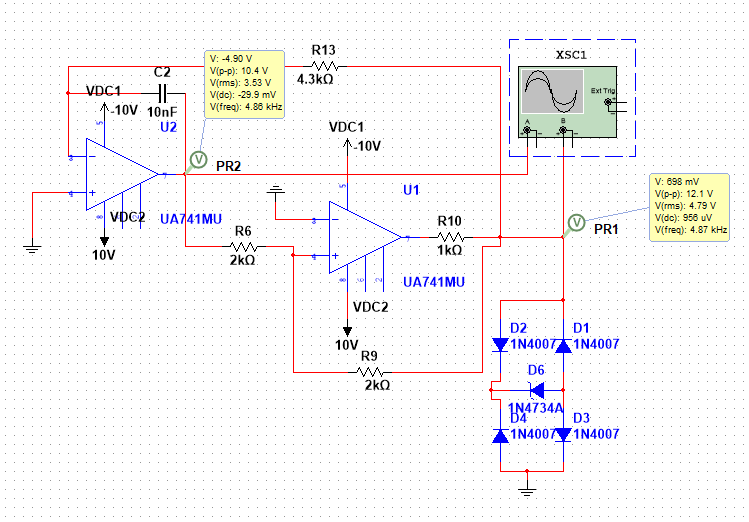
\includegraphics[width=0.8\textwidth]{simulaciones/montaje-generador-funciones.png}
    \caption{Montaje del circuito generador de funciones en multisim}
    \label{ilus:montaje-generador-funciones}
\end{ilustracion}


La ilustración \ref{ilus:montaje-generador-funciones} muestra la construcción del circuito generador de funciones utilizando los valores calculados.

\begin{ilustracion}[ht]
    \centering
    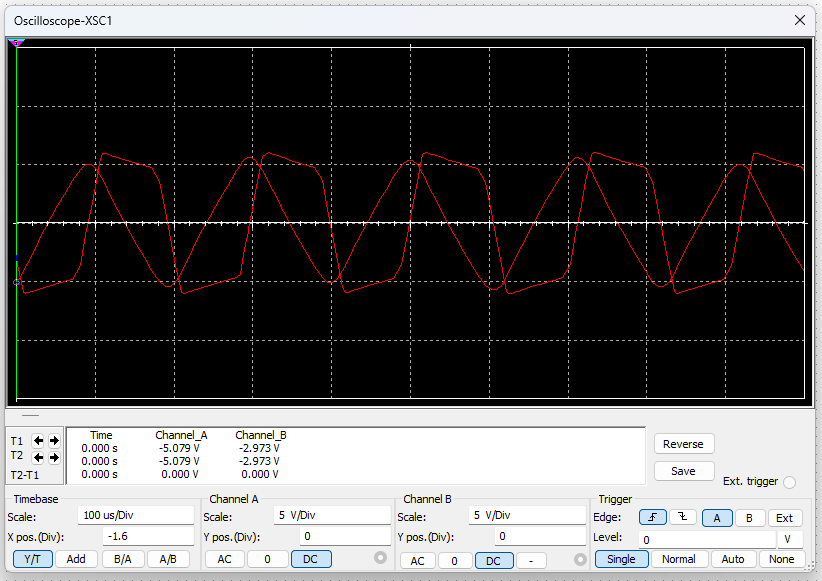
\includegraphics[width=0.9\textwidth]{simulaciones/salidas-generador-funciones.png}
    \caption{Formas de ondas triangular y cuadrada del generador de funciones en la simulación}
    \label{ilus:salidas-generador-funciones}
\end{ilustracion}

La ilustración \ref{ilus:salidas-generador-funciones} muestra las formas de onda triangular y cuadrada generadas por el circuito en la simulación. Se puede observar que la frecuencia de las ondas es de aproximadamente 5kHz y que ambas ondas tienen magnitudes casi identicas, sin embargo las magnitudes son de máximo de 6V mientras que en los calculos la magnitud era de 7.8V. También se puede observar que la señal $V_c$ no es del todo cuadrada y que la señal $V_t$ tampoco es del todo triangular.